\chapter{Ergebnisse}
\label{ch:results}

\newcommand{\regex}{\textit{regex}}
\newcommand{\llm}{\textit{llm}}
\newcommand{\json}{\textit{json}}

\newcommand{\regexv}{{\regex}-Verfahren}
\newcommand{\llmv}{{\llm}-Verfahren}
\newcommand{\jsonv}{{\json}-Verfahren}

% -------------------------------------------------------------------
% Einleitung
% -------------------------------------------------------------------

% Bezug auf die Fragestellung der Arbeit
In diesem Kapitel werden die Resultate präsentiert, die zur Beantwortung der folgenden Fragestellung dienen:

\begin{center}
    \itshape
    In welchem Umfang sind ausgewählte Llama 3 Modelle in der Lage, akkurate Koordinaten für Städte anzugeben und Distanzen zwischen Städten zu bestimmen?
\end{center}

% Übersicht über das Kapitel
Zunächst werden die Resultate des Experiments \textit{Koordinaten} (\ref{methods_coords}) präsentiert.
Zu diesem Zweck werden zu Beginn die Fehler der verschiedenen Modelle und der verschiedenen Vorlagen ohne die Länderinformation quantitativ miteinander verglichen.
Im Anschluss daran wird erörtert, welchen Einfluss die Hinzunahme des Landes hat.
Abschließend werden qualitative Beispiele vorgestellt und häufige Fehler und Probleme präsentiert.

Im weiteren Verlauf werden die Resultate des Experiments \textit{Distanz} (\ref{methods_dist}) dargestellt.
Für dieses Experiment erfolgt ebenso zunächst eine quantitative Analyse der Fehler der verschiedenen Modelle und der verschiedenen Vorlagen ohne Länderinformation.
Im Anschluss daran wird der Einfluss der Länderinformation untersucht.
Schließlich werden qualitative Beispiele vorgestellt und häufige Fehler und Probleme illustriert.

% -------------------------------------------------------------------
% Inhalt: Koordinaten
% -------------------------------------------------------------------
\section{Koordinaten}
\label{results_coords}
% Einleitung: Was wird gemacht?
Im Folgenden werden die Ergebnisse des Experiments \textit{Koordinaten} dargestellt, die aus der in Kapitel \ref{methods_coords} beschriebenen Vorgehensweise resultieren.

\subsection{Quantitativer Vergleich der verschiedenen LLMs und Verfahren}
% Allg. Informationen zur Auswertung
Bei den Auswertungen und Visualisierungen in diesem Kapitel wird häufig der durchschnittliche Fehler dargestellt.
Damit ist der durchschnittliche Fehler aller Antworten gemeint, die die angegebenen Bedingungen erfüllen, d.\,h. z.\,B. alle Antworten des Llama-3.3-70B-Instruct Modells mit dem \jsonv{} und den Länderinformationen.
Dabei werden die fehlerhaften Antworten der LLMs nicht berücksichtigt.

\subsubsection*{Ohne die Länderinformation}

\begin{figure}[tb] % Fehler der Modelle mit den Verfahren (ohne Land)
    \centering
    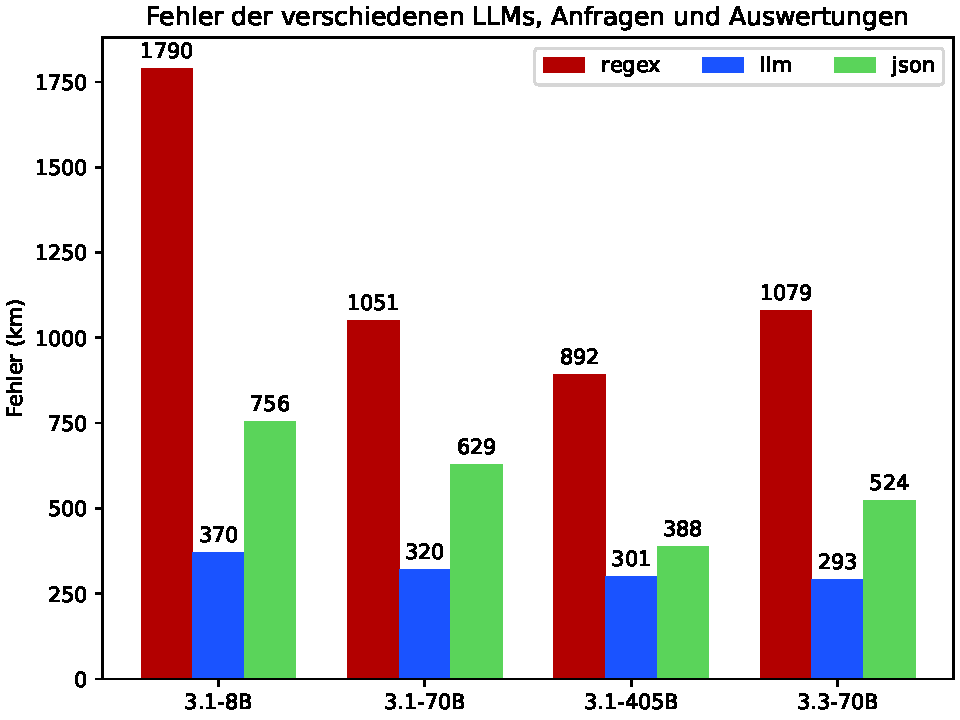
\includegraphics[width=0.7\columnwidth]{img/size_template_error_no_std.pdf}
    \caption{Der durchschnittliche Fehler von den verschiedenen LLMs, Anfragen und Auswertungsverfahren ohne die Länderinformation für das Experiment \textit{Koordinaten} (\ref{methods_coords}). Dabei werden die Fehler für die LLMs Llama-3.1-Instruct in den Größen 8B, 70B, 405B und Llama-3.3-70B-Instruct (links nach rechts) für jeweils die Auswertungsverfahren \regex{} (rot), \llm{} (blau) und \json{} (grün) mit den zugehörigen Vorlagen visualisiert.}
    \label{fig_res_coords_error}
\end{figure}

% Reihenfolge: regex > json > llm
Der durchschnittliche Fehler der Anfragen ohne zusätzliche Länderinformationen zeigt, dass für alle betrachteten Modelle das \llmv{} am besten und das \regexv{} am schlechtesten ist, während das \jsonv{} zwischen den beiden anderen liegt.
Dabei fällt auf, dass der Abstand zwischen dem \regex{}- und dem \jsonv{} größer ist als zwischen dem \llm{}- und dem \jsonv{} (vgl. Abbildung \ref{fig_res_coords_error}).

% Größe ist gut
Außerdem zeigt die Abbildung \ref{fig_res_coords_error}, dass für alle betrachteten Verfahren die Genauigkeit bei größeren Modellen zunimmt.
Die einzige Ausnahme stellt das Llama-3.3-70B-Instruct Modell mit dem \llmv{} dar, welches für dieses Verfahren die besten Ergebnisse liefert.

\begin{figure}[tb] % p-Werte für ohne Land
    \centering
    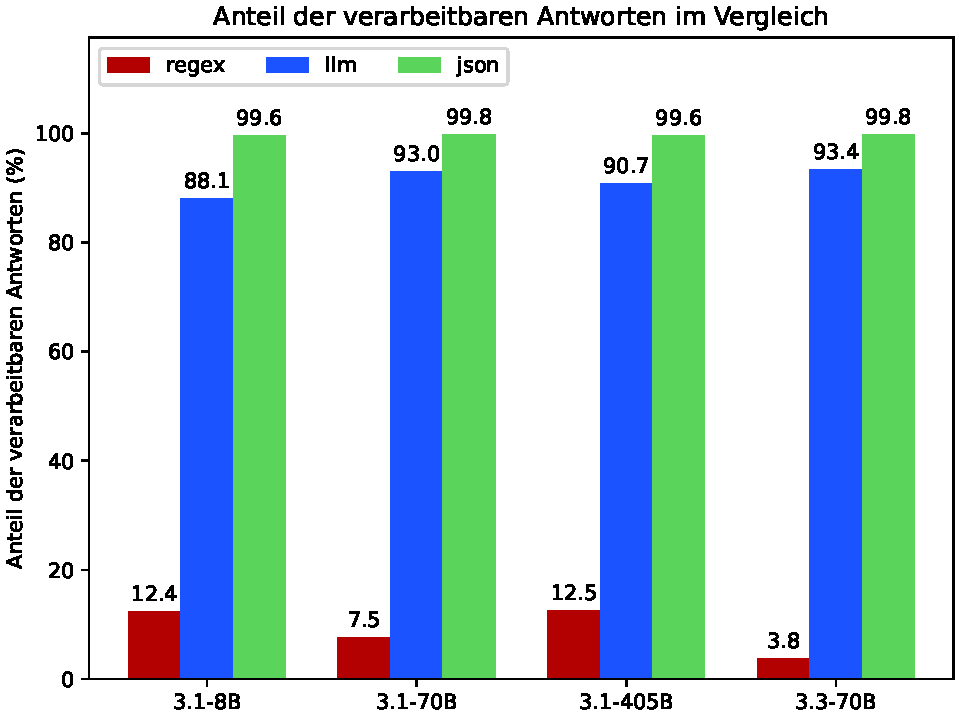
\includegraphics[width=0.7\columnwidth]{img/size_template_p.pdf}
    \caption{Der Anteil der korrekt verarbeitbaren Antworten der verschiedenen LLMs, Anfragen und Auswertungsverfahren für das Experiment \textit{Koordinaten} (\ref{methods_coords}) ohne die Länderinformationen. Dabei werden die Anteile der Antworten, die korrekt verarbeitet werden können, von den LLMs Llama-3.1-Instruct in den Größen 8B, 70B, 405B und Llama-3.3-70B-Instruct (links nach rechts) für jeweils die Auswertungsverfahren \regex{} (rot), \llm{} (blau) und \json{} (grün) mit den zugehörigen Vorlagen visualisiert.}
    \label{fig_res_coords_p}
\end{figure}

% p-Wert
% ----------------
% regex: 9.04 3.63
% llm: 91.3 2.1
% json: 99.7 0.09
% ----------------
Der Anteil der verarbeitbaren Antworten für die Anfragen ohne Länderinformationen (vgl. Abbildung \ref{fig_res_coords_p}) zeigt, dass die Verfahren unabhängig vom Modell relativ konstante Fehlerraten aufweisen.
Die Mittelwerte betragen für das \regexv{} \( \num{9.04} \pm \num{3.63} \), für das \llmv{} \( \num{91.3} \pm \num{2.1} \) und für das \jsonv{} \( \num{99.7} \pm \num{0.09} \).
Dabei fällt auf, dass das \jsonv{} nahezu fehlerfrei ist, während das \regexv{} im Durchschnitt über 90 Prozent der Anfragen so fehlerhaft beantwortet, dass es nicht möglich ist, Koordinaten zu extrahieren.

% p-Werte und Fehler passen gut zusammen
Die in den Abbildungen \ref{fig_res_coords_error} und \ref{fig_res_coords_p} dargestellten Ergebnisse weisen beide ein Muster auf.
Bei jedem Modell hat das \regexv{} eindeutig den größten durchschnittlichen Fehler und bei weitem die meisten fehlerhaften Antworten.
Im Kontrast dazu liegen das \json{}- und das \llmv{} deutlich näher beieinander.
Das \llmv{} liefert etwas bessere durchschnittliche Fehler, dafür das \jsonv{} aber nahezu keine fehlerhaften Antworten.

% Begründung: Name der Städte ist nicht eindeutig
Allerdings entstehen bei diesem Verfahren teilweise große Fehler für einzelne Städte.
Dies liegt unter anderem daran, dass Städtenamen nicht eindeutig sind.
Das führt dazu, dass Koordinaten für andere Städte mit dem gleichen Namen zurückgegeben werden.
Dies könnte der Grund dafür sein, dass z.\,B. bei dem Llama-3.1-405B-Instruct Modell mit dem \jsonv{} ohne die Länderinformation unter 1 {\%} der Anfragen für über 35 {\%} des Gesamtfehlers verantwortlich sind.
In der Abbildung \ref{fig_res_muenster_total} ist z.\,B. dargestellt, dass bei diesen Anfragen die Stadt Münster (NRW, Deutschland) wahrscheinlich mit der südlichsten Provinz Munster in Irland\footnote{\url{https://de.wikipedia.org/wiki/Munster_(Irland)}} verwechselt wurde.

\subsubsection*{Mit der Länderinformation}
Daher wird im Folgenden vorgestellt, was passiert, wenn das Land zu den Anfragen hinzugefügt wird.

\begin{figure}[tb] % Fehler der Modelle mit den Verfahren (mit Land)
    \centering
    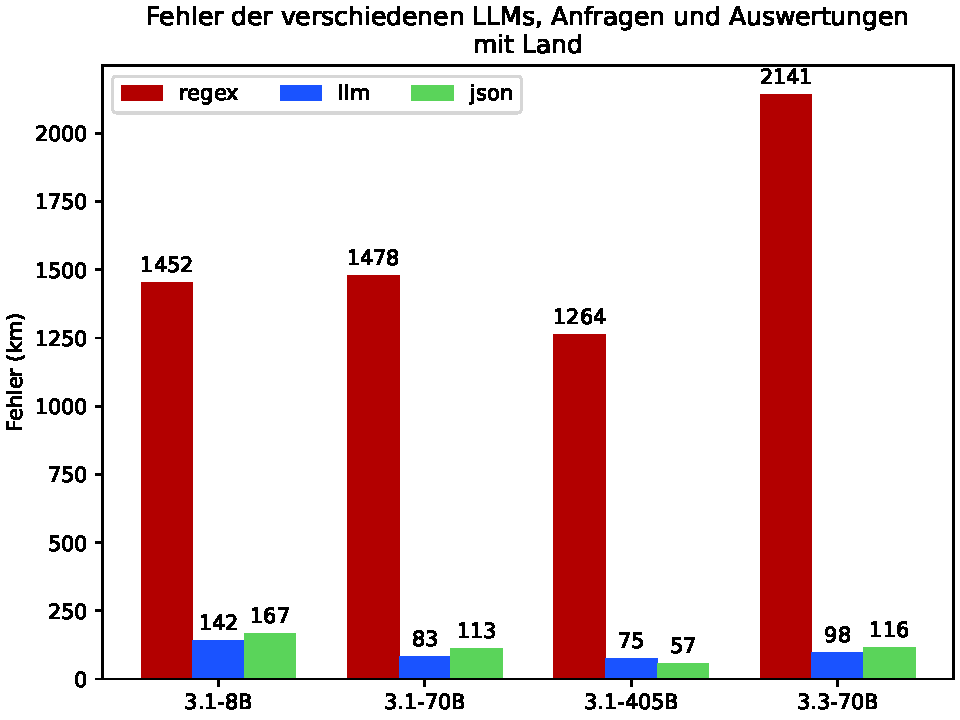
\includegraphics[width=0.7\columnwidth]{img/country_error_no_std.pdf}
    \caption{Der durchschnittliche Fehler von den verschiedenen LLMs, Anfragen und Auswertungsverfahren mit der Länderinformation für das Experiment \textit{Koordinaten} (\ref{methods_coords}). Dabei werden die Fehler für die LLMs Llama-3.1-Instruct in den Größen 8B, 70B, 405B und Llama-3.3-70B-Instruct (links nach rechts) für jeweils die Auswertungsverfahren \regex{} (rot), \llm{} (blau) und \json{} (grün) mit den zugehörigen Vorlagen visualisiert.}
    \label{fig_res_coords_error_country}
\end{figure}

% regex > json > llm
Der durchschnittliche Fehler der Anfragen mit der Länderinformation (vgl. Abbildung \ref{fig_res_coords_error_country}) zeigt ein ähnliches Muster wie der durchschnittliche Fehler der Anfragen ohne die Länderinformationen (vgl. Abbildung \ref{fig_res_coords_error}).
Bei beiden Arten der Anfragen ist das \regexv{} am schlechtesten, wobei der Abstand bei den Anfragen mit der Länderinformation deutlich angestiegen ist.
Außerdem schneidet bei beiden das \llmv{} am besten ab und das \jsonv{} liegt in der Mitte.
Ein Ausreißer sind die Anfragen mit der Länderinformation für das Llama-3.1-405B-Instruct Modell.
Hier liefert das \jsonv{} etwas bessere Ergebnisse als das \llmv{}.

% Größe ist gut, außer bei regex
Außerdem zeigt die Abbildung \ref{fig_res_coords_error_country}, dass bei den \json{}- und \llmv{} die Genauigkeit der Antworten für größere Modelle zunimmt.

\begin{figure}[tb] % p-Werte für mit Land
    \centering
    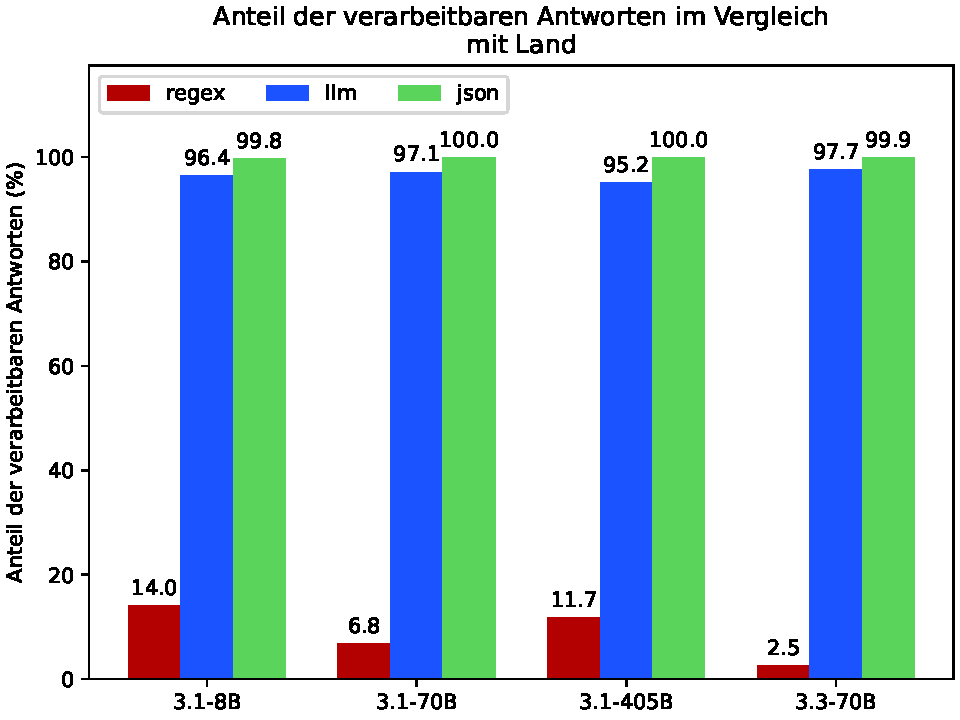
\includegraphics[width=0.7\columnwidth]{img/country_p.pdf}
    \caption{Der Anteil der korrekt verarbeitbaren Antworten der verschiedenen LLMs, Anfragen und Auswertungsverfahren für das Experiment \textit{Koordinaten} (\ref{methods_coords}) mit der Länderinformation. Dabei werden die Anteile der Antworten, die korrekt verarbeitet werden können, von den LLMs Llama-3.1-Instruct in den Größen 8B, 70B, 405B und Llama-3.3-70B-Instruct (links nach rechts) für jeweils die Auswertungsverfahren \regex{} (rot), \llm{} (blau) und \json{} (grün) mit den zugehörigen Vorlagen visualisiert.}
    \label{fig_res_coords_p_country}
\end{figure}

% p-Wert
% ----------------
% regex: 8.76 4.46
% llm: 96.6 0.95
% json: 99.91 0.09
% ----------------
Der Anteil der verarbeitbaren Antworten verändert sich durch die Hinzunahme der Länderinformation kaum (vgl. Abbildungen \ref{fig_res_coords_p} und \ref{fig_res_coords_p_country}).
Dabei bleiben die Fehlerraten für die verschiedenen Verfahren unabhängig von der Modellgröße relativ konstant; das \regexv{} sehr fehleranfällig, das \llmv{} sehr gut und das \jsonv{} praktisch perfekt.
Die Mittelwerte betragen für das \regexv{} \( \num{8.76} \pm \num{4.46} \), für das \llmv{} \( \num{96.6} \pm \num{0.95} \) und für das \jsonv{} \( \num{99.91} \pm \num{0.09} \).

% p-Werte und Fehler passen gut zusammen?
Durch Hinzunahme des Landes bei den Anfragen ändert sich nicht, dass das \regexv{} den größten Fehler und mit Abstand die wenigsten zulässigen Antworten produziert und die beiden anderen Verfahren relativ nah beisammen sind.

\subsubsection*{Auswirkungen der Hinzunahme der Länderinformation}

\begin{figure}[tb] % country vs. no country
    \centering
    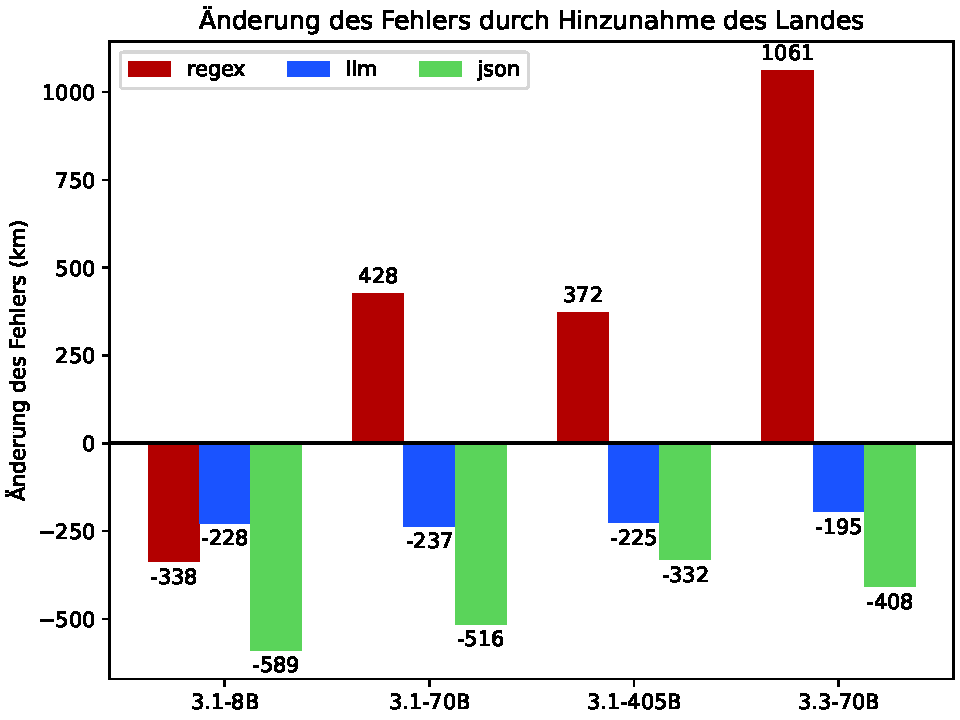
\includegraphics[width=0.7\columnwidth]{img/country_vs_no_country.pdf}
    \caption{Die Differenz zwischen den in den Abbildungen \ref{fig_res_coords_error} und \ref{fig_res_coords_error_country} dargestellten Ergebnissen des Experiments \textit{Koordinaten} (\ref{methods_coords}). Dadurch wird der Einfluss der Länderinformation in den Anfragen dargestellt. Ein negativer Wert bedeutet in dem Fall, dass der Fehler durch die Hinzunahme der Länderinformation um diesen Wert kleiner geworden ist.}
    \label{fig_res_coords_country}
\end{figure}

% -------------------------------------------------------------
% regex: \( \SI{-40.48}{\percent} \pm \num{41.45} \) Prozentpunkte
% llm: \( \SI{69.27}{\percent} \pm \num{5.49} \) Prozentpunkte
% json: \( \SI{80.83}{\percent} \pm \num{3.15} \) Prozentpunkte
% -------------------------------------------------------------

% Differenz
Die Differenz zwischen den Ergebnissen des Experiments \textit{Koordinaten} (\ref{methods_coords}) ohne die Länderinformation (vgl. Abbildung \ref{fig_res_coords_error}) und mit der Länderinformation (vgl. Abbildung \ref{fig_res_coords_error_country}) ist in der Abbildung \ref{fig_res_coords_country} dargestellt.
Anhand der Abbildung lässt sich erkennen, dass die Länderinformation keine einheitliche und tendenziell eine verschlechternde Wirkung auf das \regexv{} hat.
Bei den anderen beiden Verfahren werden die Ergebnisse durch die Hinzunahme des Landes für jedes Modell besser.
Dabei fällt auf, dass die Verbesserung für das \jsonv{} bei jedem Modell größer ist, als beim \llmv{}.
Das sorgt dafür, dass die Differenz der Fehler der \json{}- und \llmv{} nach Hinzunahme der Länderinformation deutlich kleiner geworden ist (vgl. Abbildungen \ref{fig_res_coords_error} und \ref{fig_res_coords_error_country}).

\subsubsection*{Standardabweichung}
Allerdings fällt auf, dass die Standardabweichung für alle Modelle und alle Anfragearten sehr hoch ist und sich relativ zum durchschnittlichen Fehler durch die Hinzunahme der Länderinformation kaum ändert (vgl. Abbildung \ref{fig_std_total}).

\begin{figure} % Fehler mit und ohne Länderinformation mit std
    \centering
    \begin{subfigure}{.5\textwidth}
      \centering
      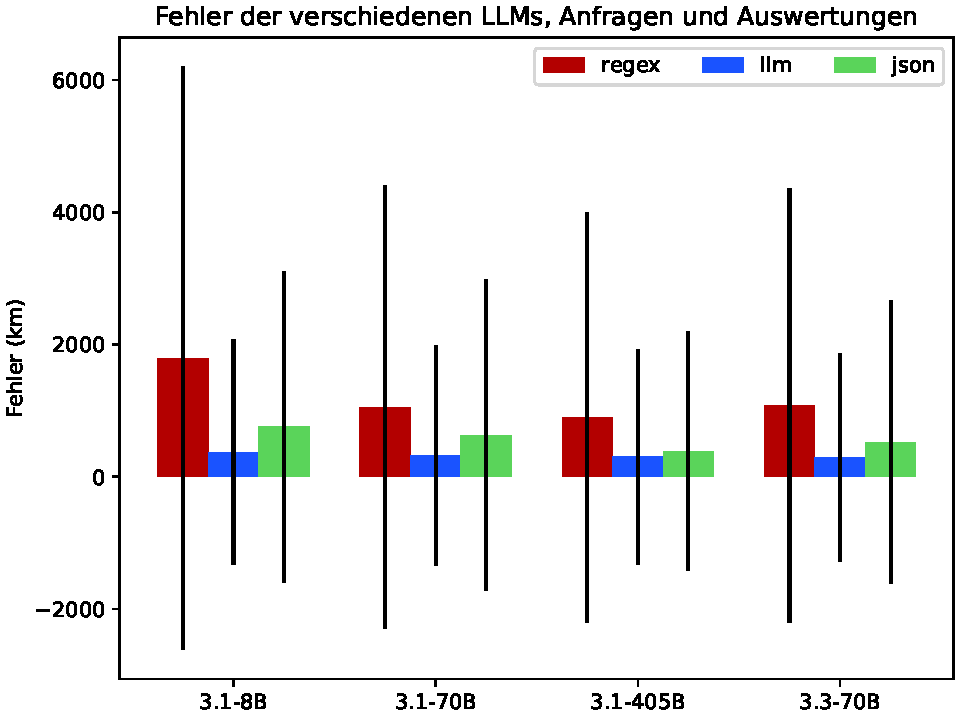
\includegraphics[width=.95\linewidth]{img/size_template_error.pdf}
      \caption{Ohne die Länderinformation.}
      \label{fig_std_without_country}
    \end{subfigure}%
    \begin{subfigure}{.5\textwidth}
      \centering
      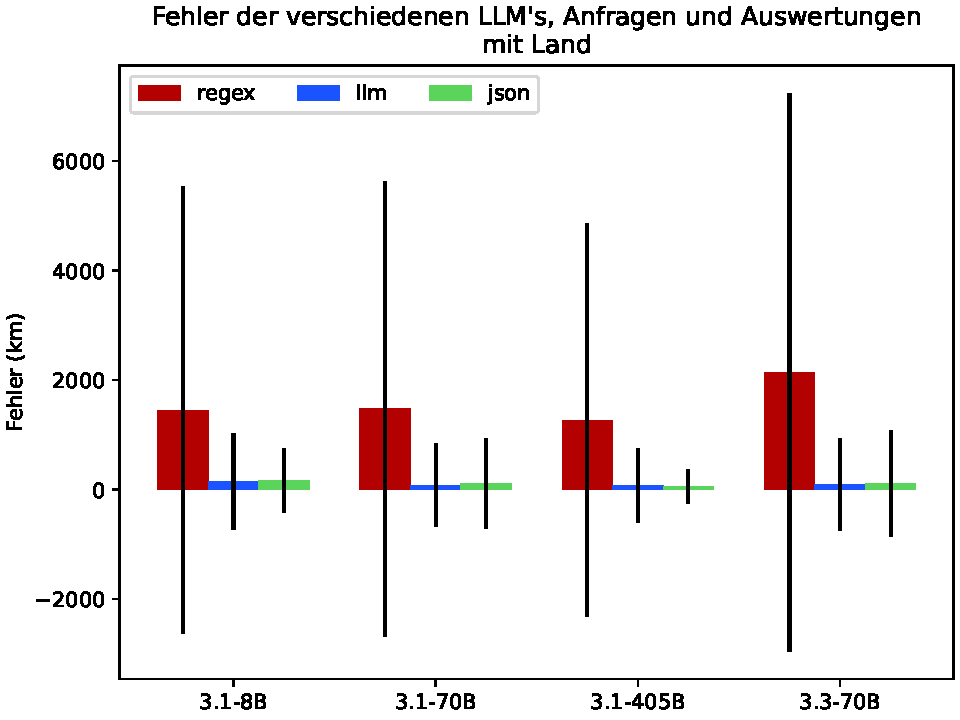
\includegraphics[width=.95\linewidth]{img/country_error.pdf}
      \caption{Mit der Länderinformation.}
      \label{fig_std_with_country}
    \end{subfigure}
    \caption{Der durchschnittliche Fehler von den verschiedenen LLMs, Anfragen und Auswertungsverfahren einmal mit und einmal ohne die Länderinformation für das Experiment \textit{Koordinaten} (\ref{methods_coords}). Dabei werden die Fehler für die LLMs Llama-3.1-Instruct in den Größen 8B, 70B, 405B und Llama-3.3-70B-Instruct (links nach rechts) für jeweils die Auswertungsverfahren \regex{} (rot), \llm{} (blau) und \json{} (grün) mit den zugehörigen Vorlagen visualisiert. Zusätzlich wird außerdem die Standardabweichung für jeden Anfragetypen in schwarz visualisiert.}
    \label{fig_std_total}
\end{figure}

\subsection{Qualitative Beispiele und Erörterung}
Im Folgenden werden einzelne Anfragen qualitativ genauer betrachtet, um das Verhalten der LLMs bei den verschiedenen Anfragearten und häufige Fehler darzustellen.

Für die Unterkapitel \textit{Ablauf und Probleme} der verschiedenen Verfahren wird das Llama-3.1-8B-Instruct Modell mit Anfragen für Abu Dhabi ohne die Länderinformation genutzt.
Außerdem werden die in Kapitel \ref{ch:methods} beschriebenen System Prompts und Vorlagen genutzt, um die Anfragen zu generieren.

\subsubsection*{Ablauf und Probleme: \regexv{}}
% Normaler Ablauf bei regex
Bei dem \regexv{} wird eine Vorlage verwendet, die kein Antwortformat vorschreibt (vgl. Abbildung \ref{fig_template_original}).
Dadurch entsteht die längere Antwort \ref{answer_original}. Trotz der Tatsache, dass die Antwort offensichtlich Koordinaten enthält, schafft es das \regexv{} nicht, Koordinaten zu extrahieren und damit einen Fehler zu berechnen.
Das kommt sehr häufig vor\footnote{Da das \regex{}- und \llmv{} dieselben Antworten auswerten, ist dies an dem Anteil der verarbeitbaren Antworten (s. Abbildung \ref{fig_res_coords_p}) erkennbar.}.

Dies ist auch das Hauptproblem des \regexv{}s.
Da aus sehr vielen Antworten fehlerhafterweise keine Koordinaten extrahiert werden, ist es nicht möglich, zuverlässige Werte zu erhalten.

\begin{figure} % Antwort für originales Template

    \begin{lstlisting}[literate={°}{\textdegree}1, breaklines=true]
        The coordinates of Abu Dhabi, the capital city of the United Arab Emirates, are:

        Latitude: 24.4653° N
        Longitude: 54.3703° E

        Please note that these coordinates are for the city center of Abu Dhabi. If you need the coordinates for a specific location within the city or the emirate, please let me know and I'll do my best to provide you with the accurate information.
    \end{lstlisting}

    \caption{Die Antwort des Llama-3.1-8B-Instruct Modells auf die Anfrage für Abu Dhabi ohne die Länderinformation mit der Vorlage \ref{fig_template_original}.}

    \label{answer_original}
\end{figure}

\subsubsection*{Ablauf und Probleme: \llmv{}}
% Normaler Ablauf bei llm
Auch das \llmv{} wertet die Antwort \ref{answer_original} aus.
Dafür wird, wie in Kapitel \ref{ch:methods} beschrieben, eine Anfrage an das Llama-3.1-8B-Instruct-Turbo Modell mit dem System Prompt \ref{fig_template_llm} und der vorigen Antwort \ref{answer_original} als Nutzereingabe gesendet.
Dabei entsteht die Antwort \ref{answer_llm}.
Diese Antwort kann sehr zuverlässig mit dem \jsonv{} ausgewertet werden.

Dabei ist das Hauptproblem, dass beim Extrahieren der Koordinaten ein anderes LLM verwendet wird.
Es kann nicht ausgeschlossen werden, dass dieses Modell fehlerhafte Koordinaten durch bessere ersetzt oder sogar bei Antworten, die keine Koordinaten enthalten, Koordinaten hinzufügt.
Allerdings zeigen die durchschnittlichen Fehler für das \llmv{} (vgl. Abbildung \ref{fig_res_coords_error}), dass das Llama-3.1-8B-Instruct Modell den größten Fehler hat.
Das lässt vermuten, dass das Llama-3.1-8B-Instruct-Turbo Modell, falls es nicht nur Koordinaten extrahieren sollte, das Ergebnis wahrscheinlich verschlechtert und nicht verbessert.

\begin{figure} % Antwort für llm-Verfahren (praktisch json-Template)

    \begin{lstlisting}[literate={°}{\textdegree}1, breaklines=true]
        {""latitude"": ""24.4653"", ""longitude"": ""54.3703""}
    \end{lstlisting}

    \caption{Die Antwort des Llama-3.1-8B-Instruct-Turbo Modells auf die Anfrage des \llmv{}s für die vorige Antwort \ref{answer_original}.}

    \label{answer_llm}
\end{figure}

\subsubsection*{Ablauf und Probleme: \jsonv{}}
% Normaler Ablauf bei json
Das \jsonv{} verwendet die Vorlage \ref{fig_template_json} und schreibt damit, genau wie die zweite Anfrage des \llmv{}s, ein festes Antwortformat vor.
Dadurch entsteht die zu der Antwort \ref{answer_llm} sehr ähnliche Antwort \ref{answer_json}.
Diese Antwort wird dann direkt ausgewertet (wie in Kapitel \ref{ch:methods} beschrieben) und der Fehler berechnet.

Dabei gibt es keine häufig auftretenden Probleme, die mit dem Verfahren zusammenhängen.

\begin{figure} % Antwort für das json-Verfahren

    \begin{lstlisting}
        {""latitude"": 24.465646, ""longitude"": 54.369824}
    \end{lstlisting}

    \caption{Die Antwort des Llama-3.1-8B-Instruct Modells auf die Anfrage für Abu Dhabi ohne die Länderinformation mit der Vorlage \ref{fig_template_json}.}

    \label{answer_json}
\end{figure}

\subsubsection*{Gleiche Städte- oder Regionennamen}
% Problem: Gleiche Städtenamen
Ein häufig auftretendes Problem ist, dass der Name einer Stadt oder Region nicht eindeutig ist, weil er z.\,B. in verschiedenen Ländern verwendet wird.
Das führt zu besonders großen Fehlern, da das LLM nur anhand des Städtenamens nicht zwischen gleichnamigen Städten unterscheiden kann und eventuell die Koordinaten einer Stadt auf einem anderen Kontinent zurückgibt, die aber nicht gemeint ist.

In Abbildung \ref{fig_res_muenster_total} wird visualisiert, dass diese Verwechselung mit dem Llama-3.1-405B-Instruct Modell bei dem \jsonv{} für die Stadt Münster (NRW, Deutschland) passiert ist.
Außerdem ist dargestellt, dass durch die Hinzunahme des Landes die Verwechselung verhindert wurde.

\begin{figure} % Karten mit Münster
    \centering
    \begin{subfigure}{.5\textwidth}
      \centering
      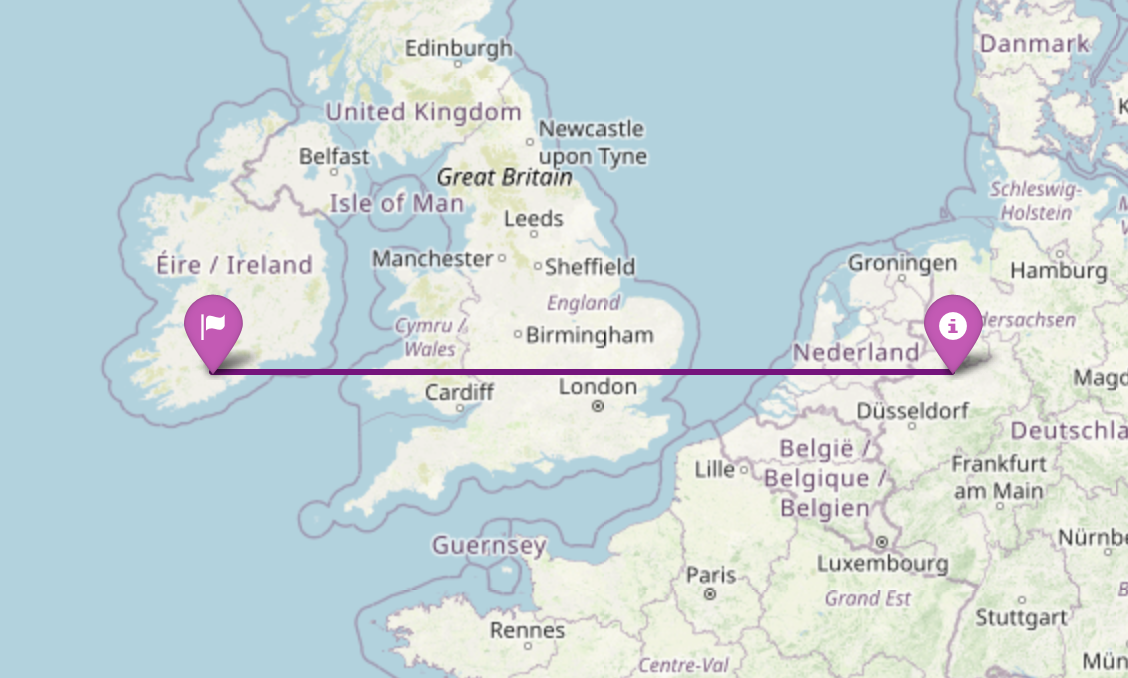
\includegraphics[width=.95\linewidth]{img/Karte-Muenster.png}
      \caption{Ohne die Länderinformation.}
      \label{fig_res_muenster}
    \end{subfigure}%
    \begin{subfigure}{.5\textwidth}
      \centering
      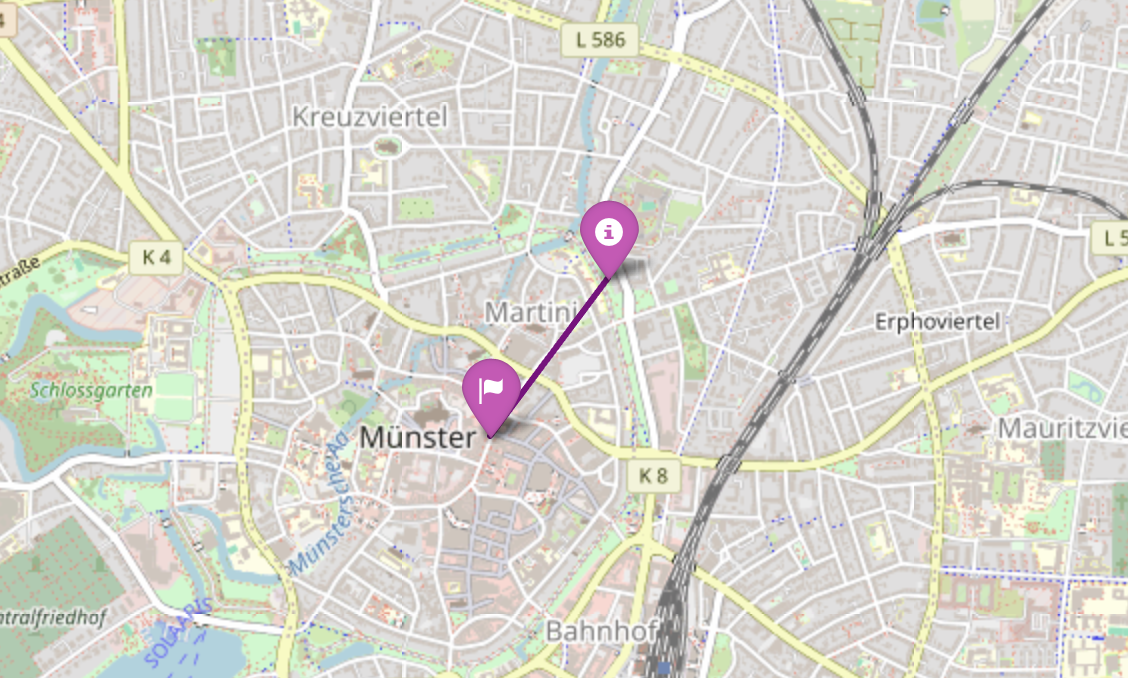
\includegraphics[width=.95\linewidth]{img/Karte-Muenster-country.png}
      \caption{Mit der Länderinformation.}
      \label{fig_res_muenster_country}
    \end{subfigure}
    \caption{Die tatsächliche Position der Stadt Münster (NRW, Deutschland) und die Ergebnisse für das Experiment \textit{Koordinaten} (\ref{methods_coords}) von dem Llama-3.1-405B-Instruct Modell mit dem \jsonv{}. Dabei wird visualisiert, welchen Einfluss die Länderinformation für die zurückgegebenen Koordinaten von Münster hat.}
    \label{fig_res_muenster_total}
\end{figure}

% Problem: Gleiche Städtenamen in einem Land
Allerdings werden dadurch nicht alle Verwechselungsprobleme gelöst.
Es kann auch vorkommen, dass innerhalb eines Landes der gleiche Städtename mehrmals verwendet wird.
Das ist für den Gesamtfehler vor allem bei großen Ländern problematisch.
In der Abbildung \ref{fig_pasadena} wird dargestellt, wie das Llama-3.1-8B-Instruct Modell mit dem \jsonv{} trotz der Länderinformation die Koordinaten für Pasadena, Kalifornien\footnote{\url{https://de.wikipedia.org/wiki/Pasadena_(Kalifornien)}} zurückgibt, obwohl Pasadena, Texas\footnote{\url{https://de.wikipedia.org/wiki/Pasadena_(Texas)}} gemeint ist.
Dadurch entsteht ein Fehler von über 2.200 km, der bei einem Durchschnittsfehler für diese Anfragen von ca. 167 km durchaus relevant ist (vgl. Abbildung \ref{fig_res_coords_error_country}).

\begin{figure}[tb] % Karte Pasadena
    \centering
    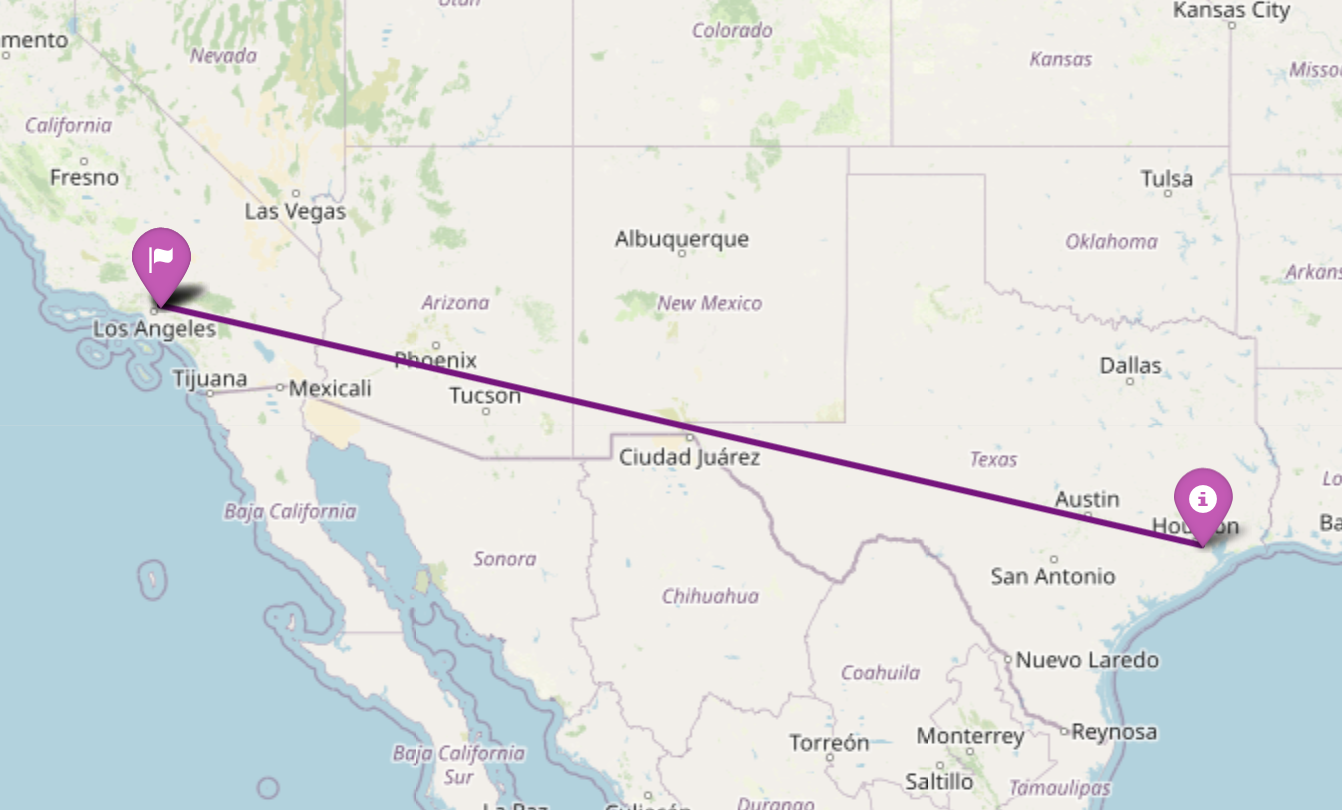
\includegraphics[width=0.7\columnwidth]{img/Karte-Pasadena.png}
    \caption{Das Llama-3.1-8B-Instruct Modell gibt mit dem \jsonv{} trotz der Länderinformation die Koordinaten für Pasadena, Kalifornien zurück, obwohl Pasadena, Texas gemeint ist.}
    \label{fig_pasadena}
\end{figure}

% -------------------------------------------------------------------
% Inhalt: Distanz
% -------------------------------------------------------------------
\section{Distanz}
\label{results_dist}
% Einleitung: Was wird gemacht?
In diesem Abschnitt werden die Resultate des Experiments \textit{Distanz} dargestellt.
Diese basieren auf der in Kapitel \ref{methods_dist} beschriebenen Vorgehensweise.

\subsection{Quantitativer Vergleich der verschiedenen LLMs}
% Was ist der Fehler
Wie bei dem vorigen Experiment wird bei den Auswertungen und Visualisierungen in diesem Kapitel meistens der durchschnittliche Fehler genutzt.
Damit ist der durchschnittliche Fehler aller Antworten gemeint, die die angegebenen Bedingungen erfüllen.
Der einzelne Fehler wird, wie in Kapitel \ref{methods_dist} beschrieben, berechnet.

\begin{figure}[tb] % Fehler Distanz mit und ohne Länderinformation
    \centering
    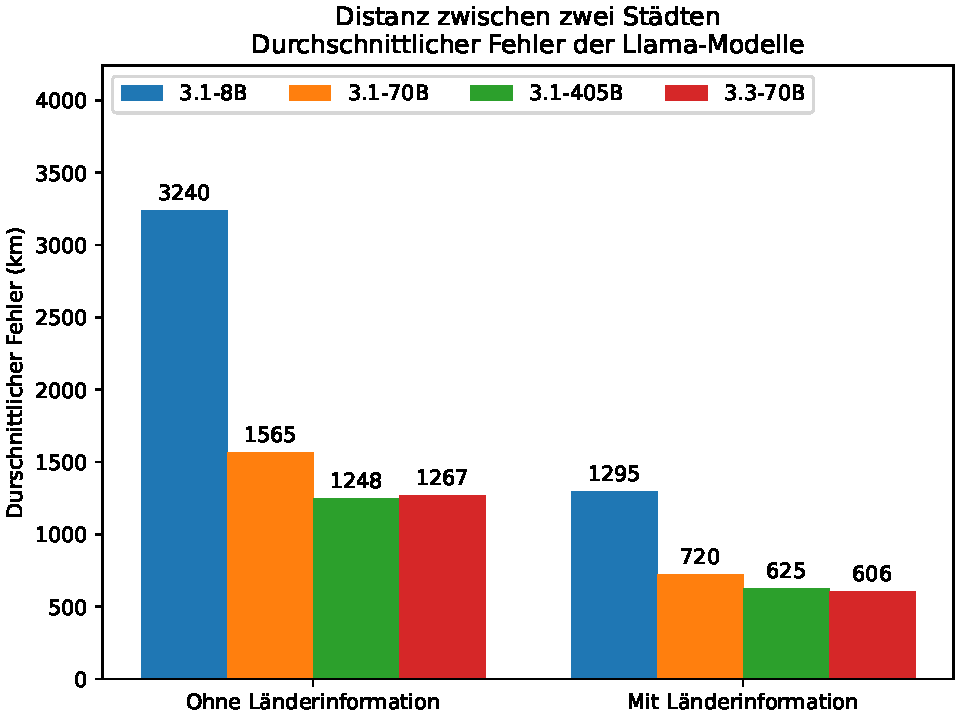
\includegraphics[width=0.7\columnwidth]{img/distance_error.pdf}
    
    \caption{
        Der durchschnittliche Fehler von den verschiedenen LLMs mit und ohne die Länderinformation für das Experiment \textit{Distanz} (\ref{methods_dist}).
        Dabei werden die Fehler für die LLMs Llama-3.1-Instruct in den Größen 8B (blau), 70B (orange), 405B (grün) und Llama-3.3-70B-Instruct (rot) einmal mit (rechts) und einmal ohne (links) die Länderinformation visualisiert.
    }

    \label{fig_dist_error}
\end{figure}

\subsubsection*{Ohne die Länderinformation}
Die durchschnittlichen Fehler ohne die Länderinformation zeigen: Je größer das LLM, desto besser das Ergebnis.
Allerdings ist der Unterschied zwischen dem Llama-3.3-70B-Instruct Modell und dem Llama-3.1-405B-Instruct Modell sehr klein (vgl. Abbildung \ref{fig_dist_error}).

\subsubsection*{Mit der Länderinformation}
Auch bei den durchschnittlichen Fehlern mit der Länderinformation zeigt sich, dass größere Modelle meistens bessere Ergebnisse produzieren (vgl. Abbildung \ref{fig_dist_error}).
Allerdings liefert das Llama-3.3-70B-Instruct Modell die besten Ergebnisse, obwohl es nicht das größte Modell ist.
Dabei muss dennoch beachtet werden, dass hier die älteren Llama 3.1 Modelle\footnote{\url{https://www.llama.com/docs/model-cards-and-prompt-formats/llama3_1/}} mit dem neueren Llama 3.3 Modell\footnote{\url{https://www.llama.com/docs/model-cards-and-prompt-formats/llama3_3/}} verglichen werden.

\subsubsection*{Auswirkungen der Hinzunahme der Länderinformation}
In Abbildung \ref{fig_dist_error} ist gut erkennbar, dass sich der Fehler durch die Hinzunahme der Länderinformation für alle Modelle ungefähr halbiert.
Dazu passt, dass sich beim Experiment \textit{Koordinaten} der Fehler für das \jsonv{} durch Hinzunahme der Länderinformation deutlich verbessert hat.

\subsubsection*{Anteil der verarbeitbaren Antworten}
% p-Werte

\begin{figure}[tb] % Distanz: p-Werte
    \centering
    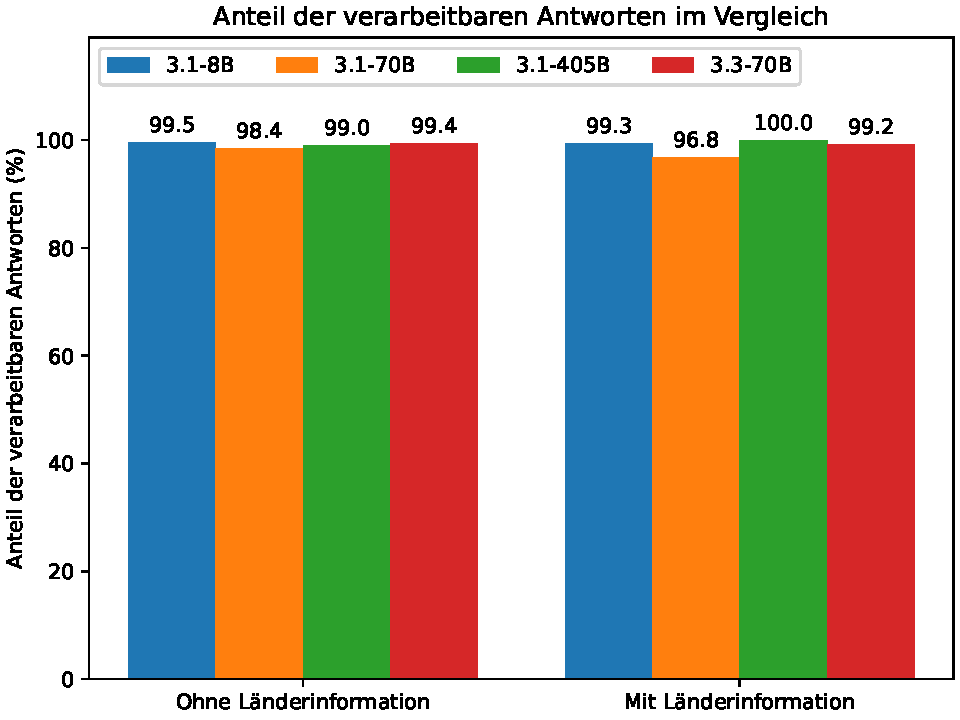
\includegraphics[width=0.7\columnwidth]{img/distance_p.pdf}
    
    \caption{
        Der Anteil der korrekt verarbeitbaren Antworten der verschiedenen LLMs mit und ohne die Länderinformation für das Experiment \textit{Distanz} (\ref{methods_dist}).
        Dabei werden die Anteile der Antworten, die korrekt verarbeitet werden können, von den LLMs Llama-3.1-Instruct in den Größen 8B (blau), 70B (orange), 405B (grün) und Llama-3.3-70B-Instruct (rot) einmal mit (rechts) und einmal ohne (links) die Länderinformation visualisiert.
    }

    \label{fig_dist_p}
\end{figure}

% ------------------------------
% Original: 99.06 +/- 0.42
% Country: 98.82 +/- 1.23
% ------------------------------

Der Anteil der verarbeitbaren Antworten ist für alle LLMs sehr groß und es gibt keine signifikanten Unterschiede (vgl. Abbildung \ref{fig_dist_p}).
Die Mittelwerte betragen für die Antworten ohne die Länderinformation \( \num{99.06} \pm \num{0.42} \) und für die Antworten mit der Länderinformation \( \num{98.82} \pm \num{1.23} \).
Diese Ergebnisse stimmen mit den nahezu perfekten Antwortraten des \jsonv{}s beim Experiment \textit{Koordinaten} überein.

\subsubsection*{Standardabweichung}
Allerdings fällt auch bei diesem Experiment auf, dass die Standardabweichung für alle Modelle sehr hoch ist.
Die Hinzunahme der Länderinformation verringert die Standardabweichung deutlich.
Trotzdem liegt die geringste Standardabweichung aller LLMs, die vom Llama-3.3-70B Modell erreicht wird, bei ca. 616 km.

\subsection{Qualitative Beispiele und Erörterung}
% Qualitativ: normale Beipsiele, Fehler (Land vs. kein Land, trotz Land falsche Stadt)
Im Folgenden wird eine einzelne Anfrage etwas genauer vorgestellt und auf Probleme eingegangen, um die Ergebnisse und die Vorgehensweise nachvollziehbarer zu machen.

\subsubsection*{Beispiel-Anfrage}
% -------------------------------------------------------------------------------------------------------
% /dev/distance-prediction/answers/llama-3.1-8B-Instruct-json-country.csv
% in,bharuch,153538,21.7,72.966667,de,berlin,3398362,52.516667000000005,13.4,6073.0307874846,"[{'role': 'system', 'content': 'Answer in json format only: {""distance"": < e.g. ""1945.399479"" >}. The value must be in kilometers and no explanation, just the answer!'}, {'role': 'user', 'content': 'What is the distance between bharuch, India and berlin, Germany?'}]","{""distance"": 6171.479892}"
% -------------------------------------------------------------------------------------------------------
Es wird die Anfrage für Bharuch, Indien und Berlin, Deutschland betrachtet.
Mithilfe der Vorlage \ref{fig_template_dist} und der Länderinformation wird die Anfrage \ref{dist_message} erstellt.
Die Antwort des Llama-3.1-8B-Instruct Modells auf diese Anfrage ist in der Abbildung \ref{dist_answer} dargestellt und entspricht einer Standardantwort für das \jsonv{}.
Mit dieser Antwort kann die Distanz direkt extrahiert werden.
In diesem Beispiel beträgt der Fehler ca. 100 km.

\begin{figure} % Anfrage für distance

    \begin{lstlisting}[literate={°}{\textdegree}1, breaklines=true]
        [
            {
                'role': 'system',
                'content': 'Answer in json format only: {""distance"": < e.g. ""1945.399479"" >}. The value must be in kilometers and no explanation, just the answer!'
            },
            {
                'role': 'user',
                'content': 'What is the distance between bharuch, India and berlin, Germany?'
            }
        ]
    \end{lstlisting}

    \caption{Die Anfrage für Bharuch, Indien und Berlin, Deutschland mit der Vorlage \ref{fig_template_dist} unter Verwendung der Länderinformation.}

    \label{dist_message}
\end{figure}

\begin{figure} % Antwort für distance

    \begin{lstlisting}[literate={°}{\textdegree}1, breaklines=true]
        {
            ""distance"": 6171.479892
        }
    \end{lstlisting}

    \caption{Die Antwort des Llama-3.1-8B-Instruct Modells für die Anfrage \ref{dist_message}.}

    \label{dist_answer}
\end{figure}

\subsubsection*{Probleme}
Die meisten Probleme, die bei dem Experiment \textit{Koordinaten} auftreten, werden hier direkt durch den Gebrauch des \jsonv{}s vermieden.
Dadurch gibt es kaum unzulässige Antworten und es besteht nicht die Möglichkeit, dass im Laufe der Auswertung die Informationen verändert werden.

Allerdings gibt es auch hier das Problem, dass die Städtenamen nicht eindeutig sind.
Das wird teilweise durch die Hinzunahme der Länderinformation behoben.
Trotzdem gibt es weiterhin das Problem gleichnamiger Städte in einem Land.

\section{Schlüsselergebnisse beider Experimente}
% Vergleich zu anderem Experiment
Bei dem Experiment \textit{Distanz} zeigen sich ähnliche Ergebnisse, wie bei dem Experiment \textit{Koordinaten}:

% \begin{samepage}
\begin{enumerate}
    \item \textbf{\jsonv{}}. Das \jsonv{} zeigt in beiden Experimenten nahezu perfekte Antwortraten -- unabhängig von der Länderinformation (vgl. Abbildungen \ref{fig_res_coords_p}, \ref{fig_res_coords_p_country} und \ref{fig_dist_p}).
    \item \textbf{Modellgröße}. In beiden Experimenten gilt, bis auf wenige Ausnahmen: Je größer das LLM, desto besser die Ergebnisse (vgl. Abbildungen \ref{fig_res_coords_error}, \ref{fig_res_coords_error_country} und \ref{fig_dist_error}).
    \item \textbf{Länderinformation}. In beiden Experimenten verbessert die Hinzunahme der Länderinformation die Ergebnisse\footnote{Ausnahme ist das \regexv{} beim Experiment \textit{Koordinaten}. Allerdings sind bei diesem Verfahren die Anteile der zulässigen Antworten so gering, dass keine zuverlässigen Werte ermittelt werden können.} (vgl. Abbildungen \ref{fig_res_coords_country} und \ref{fig_dist_error}).
\end{enumerate}

Außerdem zeigen sich bei dem Experiment \textit{Koordinaten} folgende Ergebnisse:

\begin{enumerate}
    \setcounter{enumi}{3}
    \item \textbf{\regexv{}}. Das \regexv{} erzeugt unabhängig von der Länderinformation kaum auswertbare Antworten (vgl. Abbildungen \ref{fig_res_coords_p} und \ref{fig_res_coords_p_country}).
    \item \textbf{\llmv{}}. Das \llmv{} liefert für alle LLMs, bis auf eine einzige Ausnahme, unabhängig von der Länderinformation die geringsten durchschnittlichen Fehler (vgl. Abbildungen \ref{fig_res_coords_error} und \ref{fig_res_coords_error_country}) und erzeugt kaum nicht auswertbare Antworten (vgl. Abbildungen \ref{fig_res_coords_p} und \ref{fig_res_coords_p_country}).
\end{enumerate}
% \end{samepage}